
\subsubsection{Continuum Description.}
Continuum description assumes a hypothetical continuous medium to describe behavior of a fluid/solid body. This allows description of material using continuous mathematical functions.

\subsubsection{Mechanics.}
Mechanics is classified into statics and dynamics. In crystal plasticity we study dynamics of plastic deformation. Dynamics can be further classified into Kinematics and Kinetics.

\begin{itemize}
    \item Kinematics: Study of deformation in the continuum element under consideration. Quantities measured are displacements, strains, velocities and strain rates.
    \item Kinetics: Study of forces and moments acting on the continuum object and how it affects displacements/strains or velocities/strain-rates. It involves description of material behaviour by quantification of traction/stresses and body forces using constitutive laws, material properties and conservation laws.
\end{itemize}

\section{Continuum Mechanics description of a body undergoing deformation.}

The figure \ref{Continuum_body_deformation} shows the undeformed continuum body $\mathcal{B}_0$ in reference configuration and deformed body $\mathcal{B}_t$ in current configuration. Reference configuration is time independent and current configuration is time dependent. If the deformation is described in reference/material configuration it is called Lagrangian description and if it is described in current/spatial configuration it is called Eulerian description.

Displacement at a given deformation state (at time = t) is given by,
\begin{equation}
\label{eq:A1}
    u(X) = x(X) - X
\end{equation}

A line segment $dX$ in reference configuration is transformed transformed to current configuration as,
\begin{equation}
\label{eq:A2}
    x(X) + dx = x(X) + \frac{\partial x}{\partial X}.\textrm{d}X + \textrm{O} (\textrm{d}X^2)
\end{equation}


\begin{figure}[H]
    \centering
    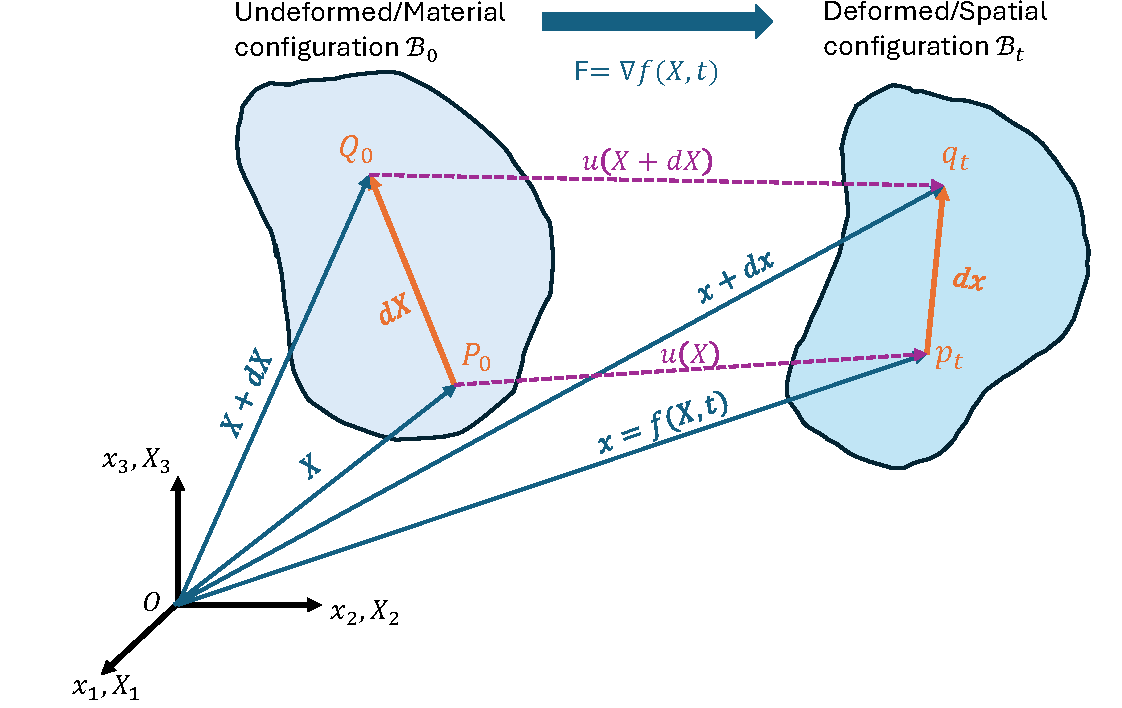
\includegraphics[width=0.9\textwidth]{images/Continuum_Mechanics_configurations.pdf}
    \caption{Deformation of a continuum body.}
    \label{Continuum_body_deformation}
\end{figure}

Neglecting higher order terms $\textrm{O} (\textrm{d}X^2)$,
\begin{equation}
\label{eq:A3}
    dx = \frac{\partial x}{\partial X}.\textrm{d}X = F.\textrm{d}X
\end{equation}

where $F:=\frac{\partial x}{\partial X}$ is called deformation gradient, a second order tensor. The deformation gradient maps the vector $\textrm{d}X$ at $X$ in the reference configuration to the vector $\textrm{d}x$ at $x$ in the current configuration. It is a 2-leg tensor because has one base at reference and one at current configuration.

From equations \ref{eq:A1} and \ref{eq:A3},
\begin{equation}
\label{eq:A4}
    F = \frac{\partial u + X}{\partial X}
\end{equation}

\begin{equation}
\label{eq:A5}
    F = I + \frac{\partial u}{\partial X}
\end{equation}

where $U:=\frac{\partial u}{\partial X}$ is called displacement gradient. Displacement gradient and deformation gradient are used to describe deformation of a body. Both are 2-leg tensors.

\section{Strain Measures}

It is possible to describe deformation only in the reference configuration as follows:

\begin{align*}
    \textrm{d}x.\textrm{d}x - \textrm{d}X.\textrm{d}X &= F.\textrm{d}X.F.\textrm{d}X -\textrm{d}X.\textrm{d}X \\
    &= \textrm{d}X.(F^T . F).\textrm{d}X - \textrm{d}X.\textrm{d}X \\
    &= \textrm{d}X.(F^T . F - I).\textrm{d}X \\
    &= \textrm{d}X.(2E_0).\textrm{d}X
\end{align*}
where $E_0 = \frac{1}{2}(F^T . F - I)$ is called Green-Lagrange strain tensor which is defined only in reference configuration.

Similarly, it is also possible to describe deformation in current configuration
\begin{align*}
    \textrm{d}x.\textrm{d}x - \textrm{d}X.\textrm{d}X &= \textrm{d}x.\textrm{d}x - F^{-1}.\textrm{d}x.F^{-1}.\textrm{d}x\\
    &= \textrm{d}x.\textrm{d}x - \textrm{d}x.(F^{-T} . F^{-1}).\textrm{d}x\\
    &= \textrm{d}x.(I - F^{-T} . F^{-1}).\textrm{d}x \\
    &= \textrm{d}X.(2E_t).\textrm{d}X
\end{align*}
this leads to definition of Euler-Almansi strain tensor $E_t = \frac{1}{2}(I - F^{-T} . F^{-1})$ which is defined only in current configuration.

Cauchy strain can be defined in terms of displacement gradient as,
\begin{equation}
    \epsilon = \frac{1}{2} \left( \nabla u + ( \nabla u)^T \right)
\end{equation}

For ONE-DIMENSION cases without lateral contraction the deformation can be described in terms of two variables: length in reference configuration $l_0$ and length in current configuration $l_t$ . By defining the ratio of these two variables as 'stretch ratio $\lambda$' we can compare the strain measures as given in the table \ref{Strain_measures_def}

\begin{table}[H]
    \centering
    \caption{Definition of strain measures for 1D cases}
    \begin{tabular}{c|cc}
        configuration & strain measure & definition in 1D \\
        \hline
        reference & Green-Lagrange strain & $E_{0,1dim = \frac{1}{2}(\lambda^2-1)}$ \\
        current & Euler-Almansi strain &  $E_{t,1dim = \frac{1}{2}(1 - \frac{1}{\lambda^2})}$ \\
        2-leg & Cauchy strain & $\epsilon_{1dim} = \lambda - 1$
    \end{tabular}
    
    \label{Strain_measures_def}
\end{table}

\section{Stress Measures}
Stress is a second order tensor defined using force and area vectors which can be defined in reference or current configuration. As a result different stress measures exist.

The stress measures along with strain measures are summarized in the table \ref{Stress_Measures_Configurations}. 

\begin{table}[H]
\centering
\caption{Stress and Strain measures in different configurations.}
\renewcommand\arraystretch{1.4}
\renewcommand\baselinestretch{1.4}
\begin{tabular}{c|ccc}
    configuration & stress & strain & symmetry \\
    \hline
    current/spatial & Cauchy Stress & Euler-Almansi strain & symmetric \\
    2-leg & 1st Piola-Kirchhoff stress & Displacement Gradient & non-symmetric\\
    reference/material & 2nd Piola-Kirchhoff stress & Green-Lagrange strain & symmetric\\
\end{tabular}

\label{Stress_Measures_Configurations}
\end{table}

The conversion between different stress measures used in DAMASK is given in table \ref{Stress_measures}

\begin{table}[H]
\centering
\caption{Conversion between different stress measures used in DAMASK.}
\renewcommand\arraystretch{1.4}
\renewcommand\baselinestretch{1.4}
\begin{tabular}{c|c|c|c}
    & $P$ (PK1)) & $S$ (PK2) & $\sigma$ (Cauchy) \\
    \hline
    $P$ & $P$ & det$F_pF_eF_iSF_p^{-T}$ & det$F\sigma F^{-T}$ \\
    $S$ & $\frac{1}{\mbox{det} F_p}F_i^{-1}F_e^{-1}PF_p^T$ & $S$ & det$(F_eF_i)F_i^{-1}F_e^{-1}\sigma F_e^{-T}F_i^{-T}$\\
    $\sigma$ & $\frac{1}{\mbox{det}F}PF^T$ & $\frac{1}{\mbox{det} (F_eF_i)}F_eF_iSF_i^{T}F_e^{T}$ & $\sigma$\\
\end{tabular}

\label{Stress_measures}
\end{table}

\section{Constitutive relation for Linear Elasticity}
Each stress components can be expressed as a linear combination of strain components in linear elasticity theory or Hooke's law, which is written as:
\begin{equation*}
    \sigma_{ij} = c_{ijkl} \epsilon_{kl}
\end{equation*}

where $c_{ijkl}$ are components of the elastic stiffness tensor. The symmetries in the strain and the stress reduce 81 different entries in the elastic tensor to 36 independent elements.
In the linear elasticity, the potential energy must be quadratic function of elastic strain. This further reduces the number of independent elements to 21.

Various crystallographic symmetries in the lattice structure reduces the number of independent elastic constants further as given in the table \ref{Independent_Cijkl}. To simplify representation of elastic constants Vogit notation is used in the below table where indices are mapped as: $11\to 1, \ 22 \to 2, \ 33 \to 3, \ 23\&32 \to 4, \ 13\&31 \to 4, \ 12\&21 \to 6$ 

\begin{table}[H]
\centering
\caption{Independent elastic constants for various crystal symmetries.}
\begin{tabular}{c m{4em} c}
    \hline
    Crystal Class & Independent $C_{ij}$ & List of independent $C_{ij}$ \\
    \hline
    Triclinic & 21 & All possible combinations \\
    Monoclinic & 13 & $C_{11}, C_{12}, C_{13}, C_{16}, C_{22}, C_{23}, C_{26}, C_{33}, C_{36}, C_{44}, C_{45}, C_{55}, C_{66}$ \\
    Orthorhombic & 9 & $C_{11}, C_{12}, C_{13}, C_{22}, C_{23}, C_{33}, C_{44}, C_{55}, C_{66}$ \\
    Trigonal & 6 or 7 & $C_{11}, C_{12}, C_{13}, C_{14}, C_{25},  C_{33}, C_{44}$ \\
    Tetragonal & 6 & $C_{11}, C_{12}, C_{13}, C_{33}, C_{44}, C_{66}$ \\
    Hexagonal & 5 & $C_{11}, C_{33}, C_{44}, C_{12}, C_{14}$ \\
    Cubic & 3 & $C_{11}, C_{12}, C_{44}$ \\
    Isotropic & 2 & $C_{11}, C_{44}$ \\
    \hline
\end{tabular}

\label{Independent_Cijkl}
\end{table}


